\title{2019 Entomology Highlights from Alaska’s Forests}

\subtitle{\doi{10.----------}}

\author{by Garret Dubois\footnoteremember{fs}{USDA Forest Service R10, Forest Health Protection}, Stephen Burr\footnoterecall{fs}, Elizabeth Graham\footnoterecall{fs}, Jason Moan\footnoteremember{dnr}{AKDNR Division of Forestry}, Jessie Moan\footnote{UAF Cooperative Extension Service}, Martin Schoofs\footnoterecall{dnr} and Steve Swenson\footnoterecall{fs}}

\maketitle

Alaska’s forest health is monitored annually by a multi-agency team with representatives from \acr{USDA} Forest Service, \acr{AKDNR} Division of Forestry and UAF Cooperative Extension Service. Our mission is to protect and enhance forest health by providing landowners and managers with information and resources. Part of our core mission is to provide technical assistance and information about forest health conditions in Alaska, including the status of many forest insect pests which is assessed through ground and aerial surveys. The results of this work are published in the annual Forest Health Conditions in Alaska report. The full report can be found at \url{https://www.fs.usda.gov/Internet/FSE_DOCUMENTS/fseprd712413.pdf}. 

\section{Spruce beetle}
Spruce beetle, \textit{Dendroctonus rufipennis}, is native to Alaska and has a long history of outbreaks particularly in Southcentral and Southwest Alaska. Outbreaks have been recorded in, but are not limited to the 1810s, 1870s, 1910s, and 1970s, usually following one or more years of warmer and drier than average summer conditions. An outbreak in Southcentral Alaska that started with sporadic activity in the 1980’s progressed in intensity and severity in the 1990s and continued into the early 2000s. This outbreak affected well over 3 million acres of forest with >90\% of the trees killed in many stands. Currently, Southcentral Alaska continues to be in the midst of a new spruce beetle outbreak (Figure \ref{spruce_beetle}), estimated to be in its fourth year. Damage has been primarily observed throughout the Matanuska-Susitna Valley areas and the central and northwest Kenai Peninsula. Elevated spruce beetle damage was first observed during annual forest health aerial detection surveys in 2015 with 33,000 acres mapped; double that from the previous year. Forest health surveyors continued to document an increase in spruce beetle damage in 2016, with nearly 200,000 acres of mapped damage, and the acreage again doubled in 2017 to 400,000 acres. In 2018 mapped damage approached 600,000 acres. Damage decreased considerably in 2019, with 139,500 acres mapped statewide during aerial surveys, though, spruce beetle activity continues to intensify in areas that were previously lightly impacted and is expanding in nearly all directions along the periphery of the outbreak area.  In some areas white spruce host material is near exhaustion and an increase in spruce beetle attacks on black spruce has been observed.

\begin{figure}[H]
\begin{center}
\vspace{2mm}
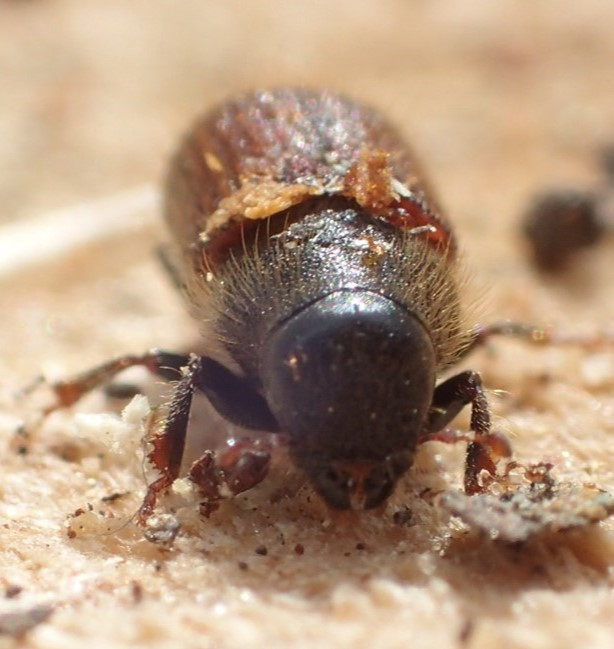
\includegraphics[width=\textwidth]{img/spruce_beetle.jpg}
\caption{Spruce beetle, \textit{Dendroctonus rufipennis}, activity is still expanding but acres mapped are dropping. Depleted host material may be having an impact.}
\label{spruce_beetle}
\end{center}
\end{figure} 

In 2017, there were a few reports of non-spruce conifers, Scots pine (\textit{Pinus sylvestris}) and Siberian larch (\textit{Laris sibirica}) being attacked by bark beetles in the Susitna River valley. From specimens collected from the attacked trees, Dr.\ James LaBonte, Insect Taxonomist with the Oregon Department of Agriculture, confirmed that spruce beetle was the species attacking these non-native non-host conifers. Many of the initial attacks on both non-native tree species appeared to have been unsuccessful, though gallery initiation was observed at several attack sites in Scots pine and in at least one attack site in Siberian larch. Lodgepole pine (\textit{Pinus contorta}) are also present in many of the locations where Scots pines have been attacked; no spruce beetle attacks have been observed in lodgepole pine to date. Observed attacks in Scots pine and Siberian larch have thus far been minimal and seemingly unsuccessful, however, heavy beetle attacks were documented in what appear to be jack pines (\textit{Pinus banksiana}), an uncommon ornamental tree in Southcentral Alaska, in 2018. Beetles collected from these affected trees were also confirmed by Dr.\ LaBonte as spruce beetles. In the spring of 2019, emergence traps were installed on these affected trees, which resulted in the collection of dozens of adult beetles, suggesting the collected beetles likely completed their life cycle in these trees. Additional investigation of the affected trees is needed to confirm this finding. 

\begin{figure}[H]
\begin{center}
\vspace{2mm}
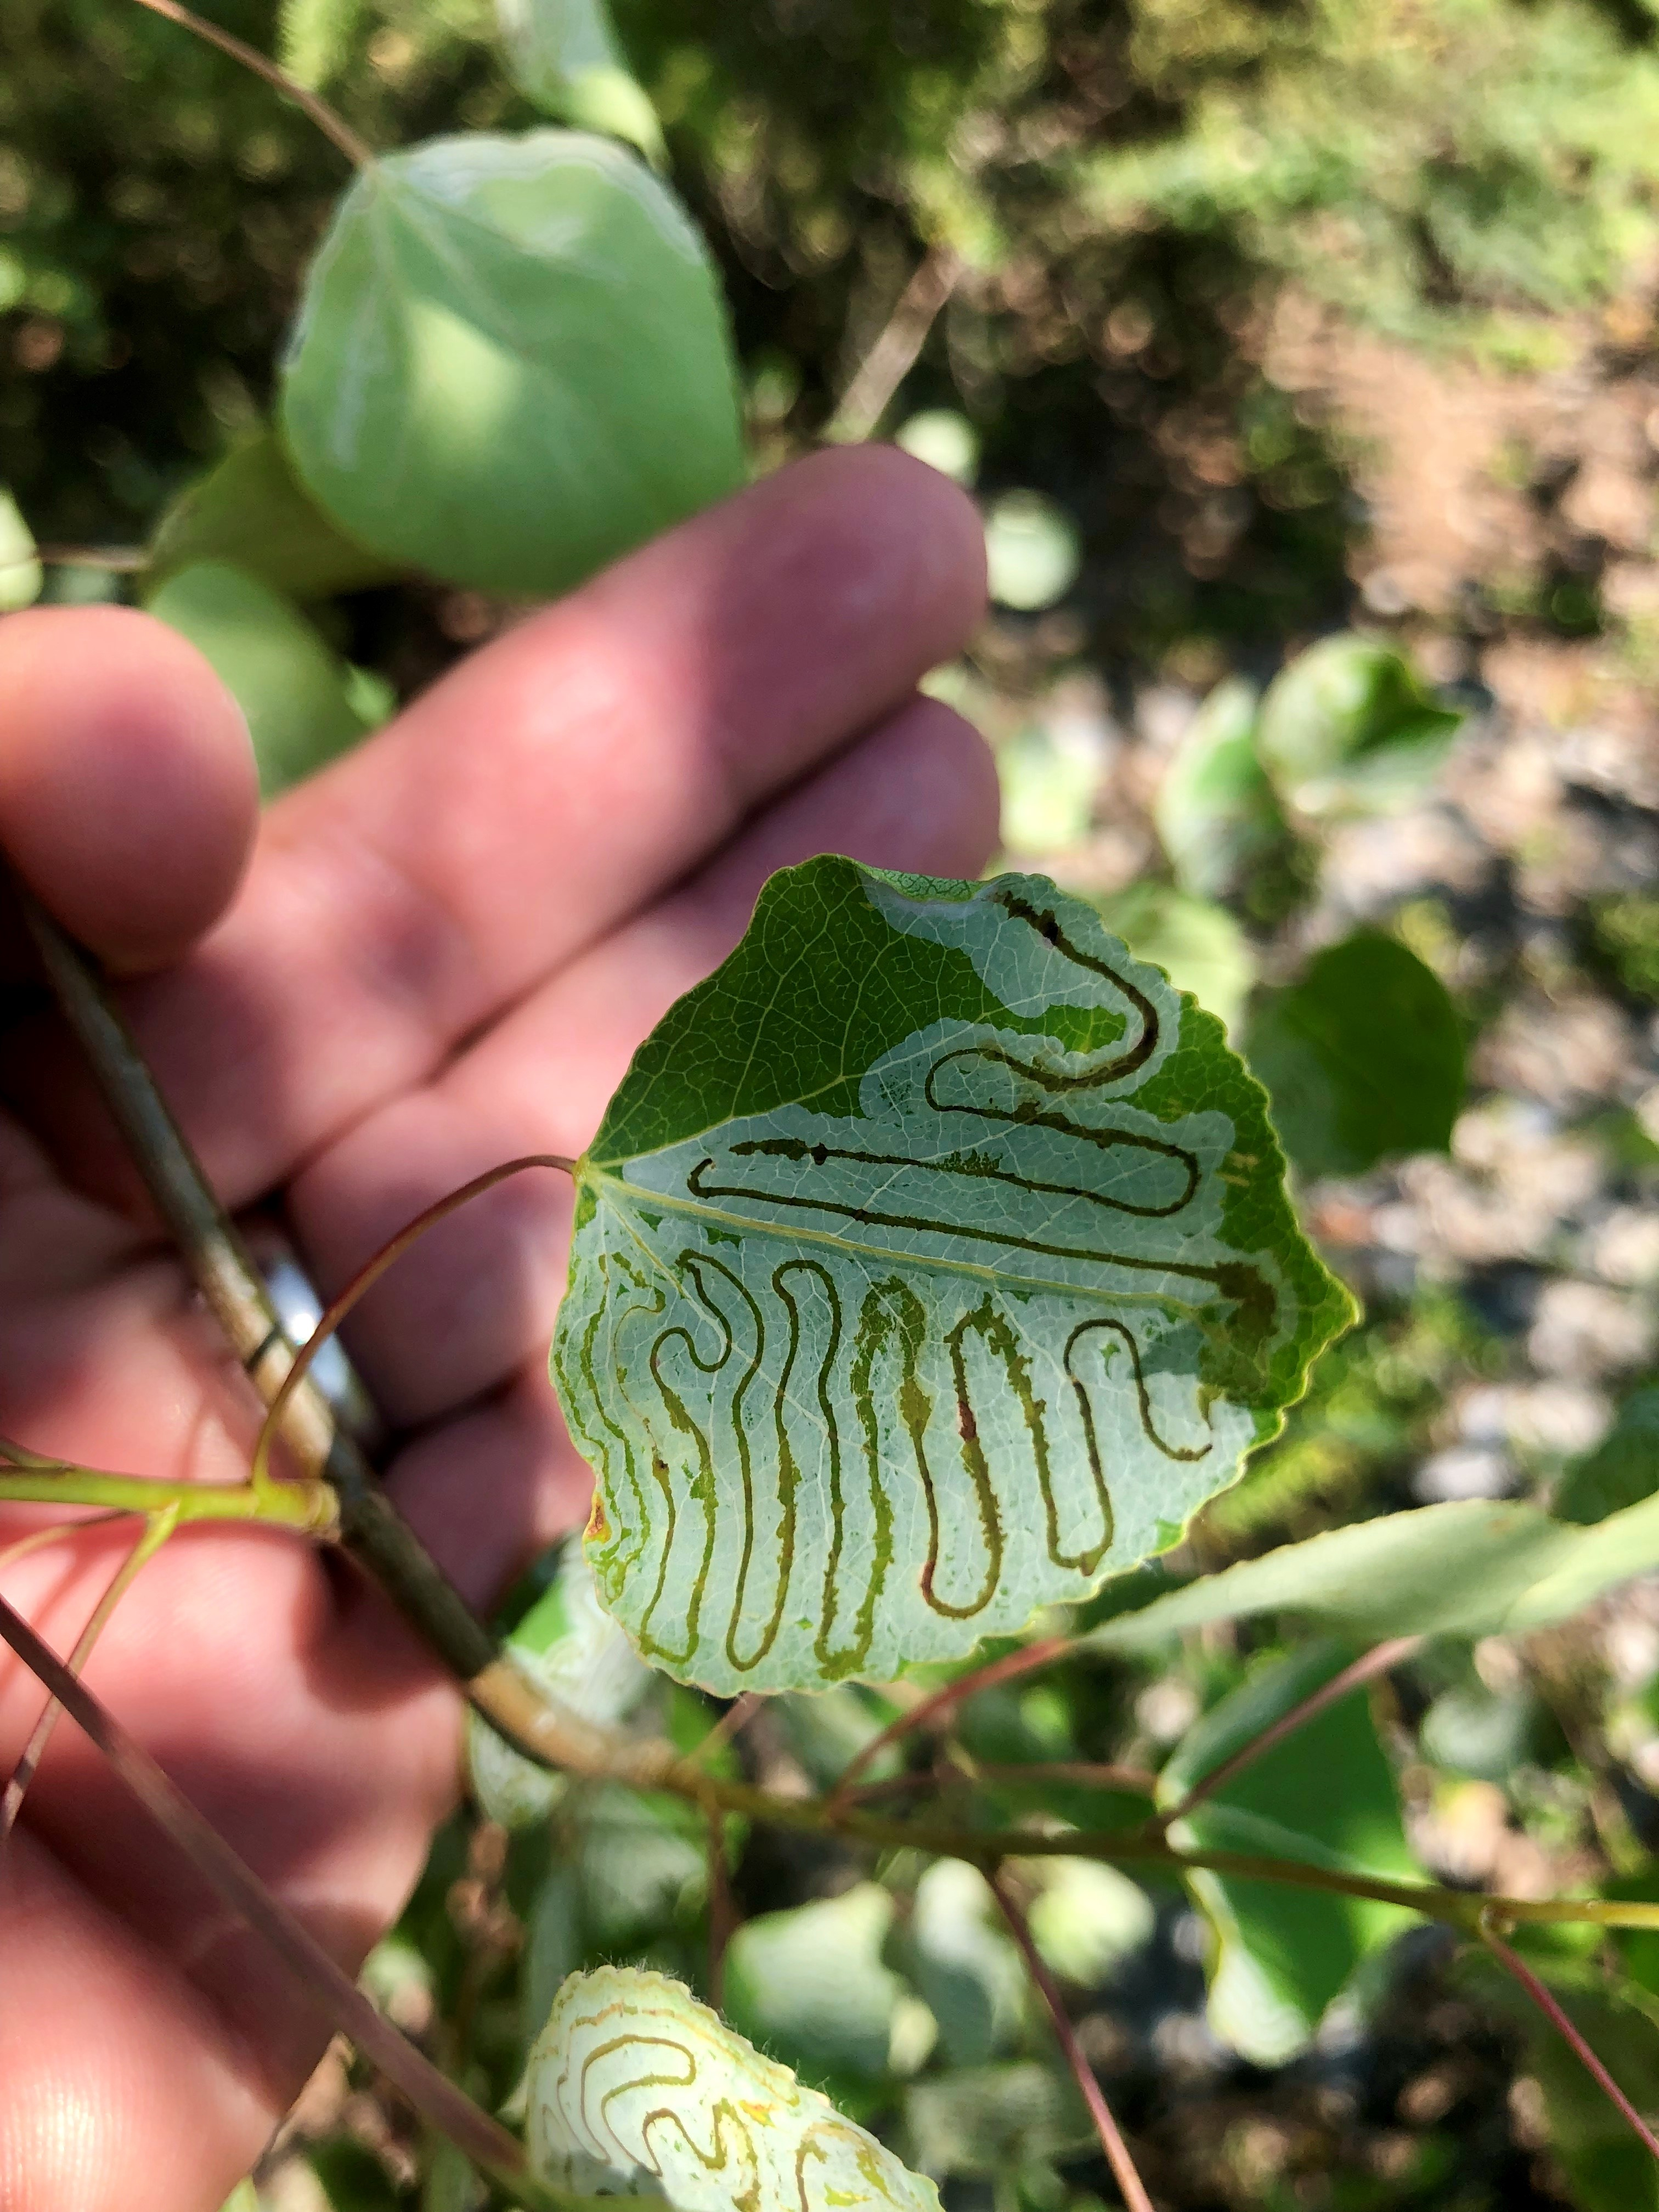
\includegraphics[width=\textwidth]{img/aspen_leafminer.jpg}
\caption{Aspen leaf miner, \textit{Phyllocnistis populiella}, is found all across the Interior Alaska, this damage was seen out on Manley Hot Springs Road.}
\label{aspen_leafminer}
\end{center}
\end{figure} 

\section{Aspen leafminer and willow leafblotch miner}

Aspen leafminer, \textit{Phyllocnistis populiella}, and willow leafblotch miner, \textit{Micurapteryx salicifoliella}, continue to be prevalent in the Interior (Figures \ref{aspen_leafminer} and \ref{willow_leafblotch_miner}) and were mapped on 132,000 and 32,000 acres respectively. Mapped acres in 2019 dropped from those recorded in the previous season for both insects, this was likely due to the difficulties encountered during aerial survey in 2019. Wildfires with vast areas of smoke and temporary flight restrictions interrupted, redirected or curtailed many aerial survey missions. Ground surveys, however, confirmed that both insects were widespread, causing heavy damage in many areas. Aspen leafminer is native to Alaska but was first observed as a problem in the 1970s and has been in outbreak in varying portions of the Interior and in the Copper River Valley since the early 2000s. Currently, aspen leafminer seems to be present in nearly every stand of aspen encountered in the Interior and is also present locally in areas around Glennallen and Copper Center. 

\begin{figure}[H]
\begin{center}
\vspace{2mm}
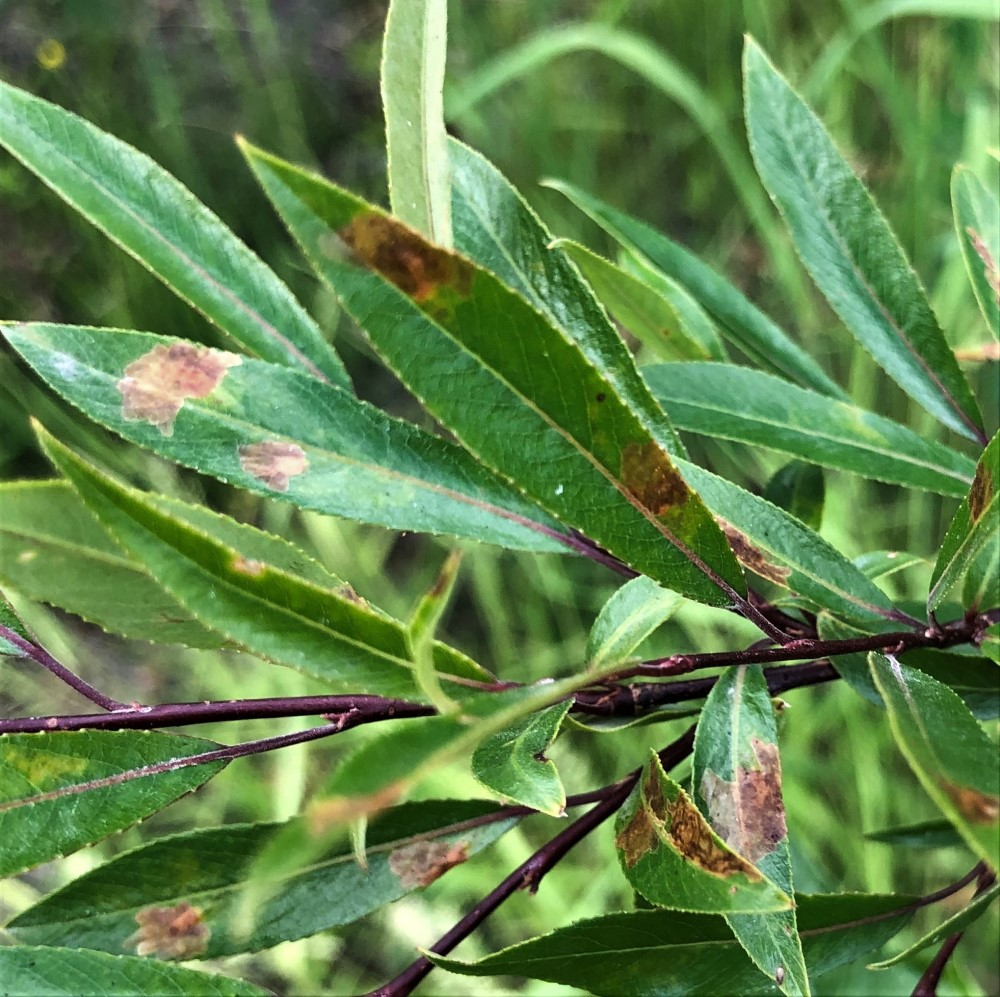
\includegraphics[width=\textwidth]{img/willow_leafblotch_miner.jpg}
\caption{Willow leafblotch miner, \textit{Micurapteryx salicifoliella}, is in many areas where willow is present. This damage was located along the Tanana River at Manley.}
\label{willow_leafblotch_miner}
\end{center}
\end{figure} 

Willow leafblotch miner is native to North America. A single specimen was identified from Bonanza Creek Experimental Forest, south of Fairbanks in the 1980s. There are no other records of willow leafblotch miner in Alaska until the early- and mid-1990s when there were several large outbreaks. Since those initial outbreaks it has been found to be causing minor to substantial damage nearly everywhere in the Interior where its host species are present. Willow leafblotch miner has been known to infest at least 10 of the 30+ species of willow in Alaska. Species like feltleaf willow are rarely attacked because of the dense layer of trichomes on the leaf surfaces that inhibit oviposition and egg attachment \citep{Furnissetal2001}. Willow leafblotch miner damage is most notable in the Interior especially in the Yukon Flats area.

\begin{figure}[H]
\begin{center}
\vspace{2mm}
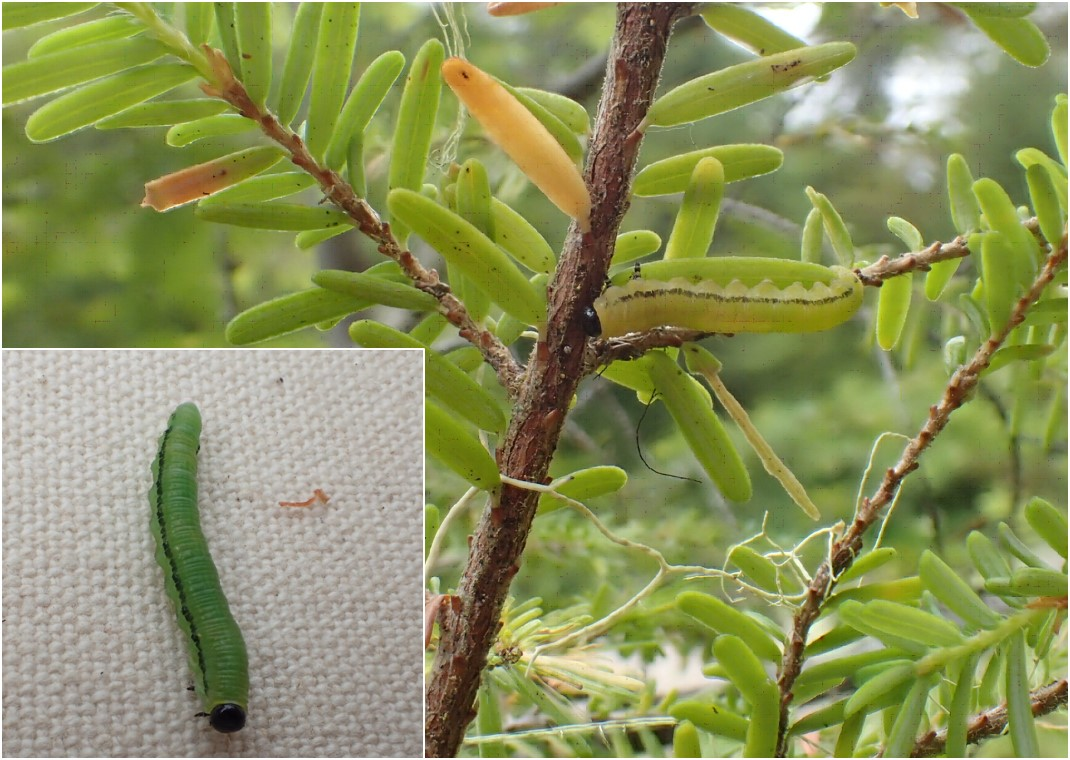
\includegraphics[width=\textwidth]{img/hemlock_sawfly.jpg}
\caption{Hemlock sawfly, \textit{Neodiprion tsugae}, larvae found in Southeast Alaska.}
\label{hemlock_sawfly}
\end{center}
\end{figure}  

\section{Hemlock sawfly}

The hemlock sawfly, \textit{Neodiprion tsugae}, is native to Alaska and population dynamics tend to be linked to entomopathogenic fungi, parasitic wasps and environmental conditions. Because of these interactions, population levels fluctuate from year to year to varying degrees. The current outbreak that began in 2018 is the first since 2013 and has continued throughout Southeast Alaska with over 380,000 acres of damage recorded during the 2019 aerial detection surveys (Figure \ref{hemlock_sawfly}), primarily to western hemlock (\textit{Tsuga heterophylla}). Defoliation is extensive in some areas, especially Prince of Wales, Mitkof, and Kupreanof Islands, and extending north to Juneau. Further details about hemlock sawfly surveys can be found in the hemlock sawfly article \citep{Graham2020}.  

\section{Birch leafminers}

In 2019, special late-season aerial surveys were scheduled in both Southcentral and Interior Alaska to better assess the impacts of the non-native and invasive birch leafminers \textit{Profenusa thomsoni} and \textit{Heterarthrus nemoratus} (Figure 5). Late season aerial surveys have allowed us to map damage that was not apparent or had not yet occurred during our standard aerial survey timing. These special survey missions have allowed us to paint a better picture of the severity and extent of the birch leafminer damage, particularly off the road system. Over 280,000 acres of impacted forests were mapped in 2019; 17,000 acres in Interior, over 170,000 acres in the Matanuska-Susitna Borough and more than 80,000 acres on the northern Kenai Peninsula. 

\begin{figure}[H]
\begin{center}
%\vspace{2mm}
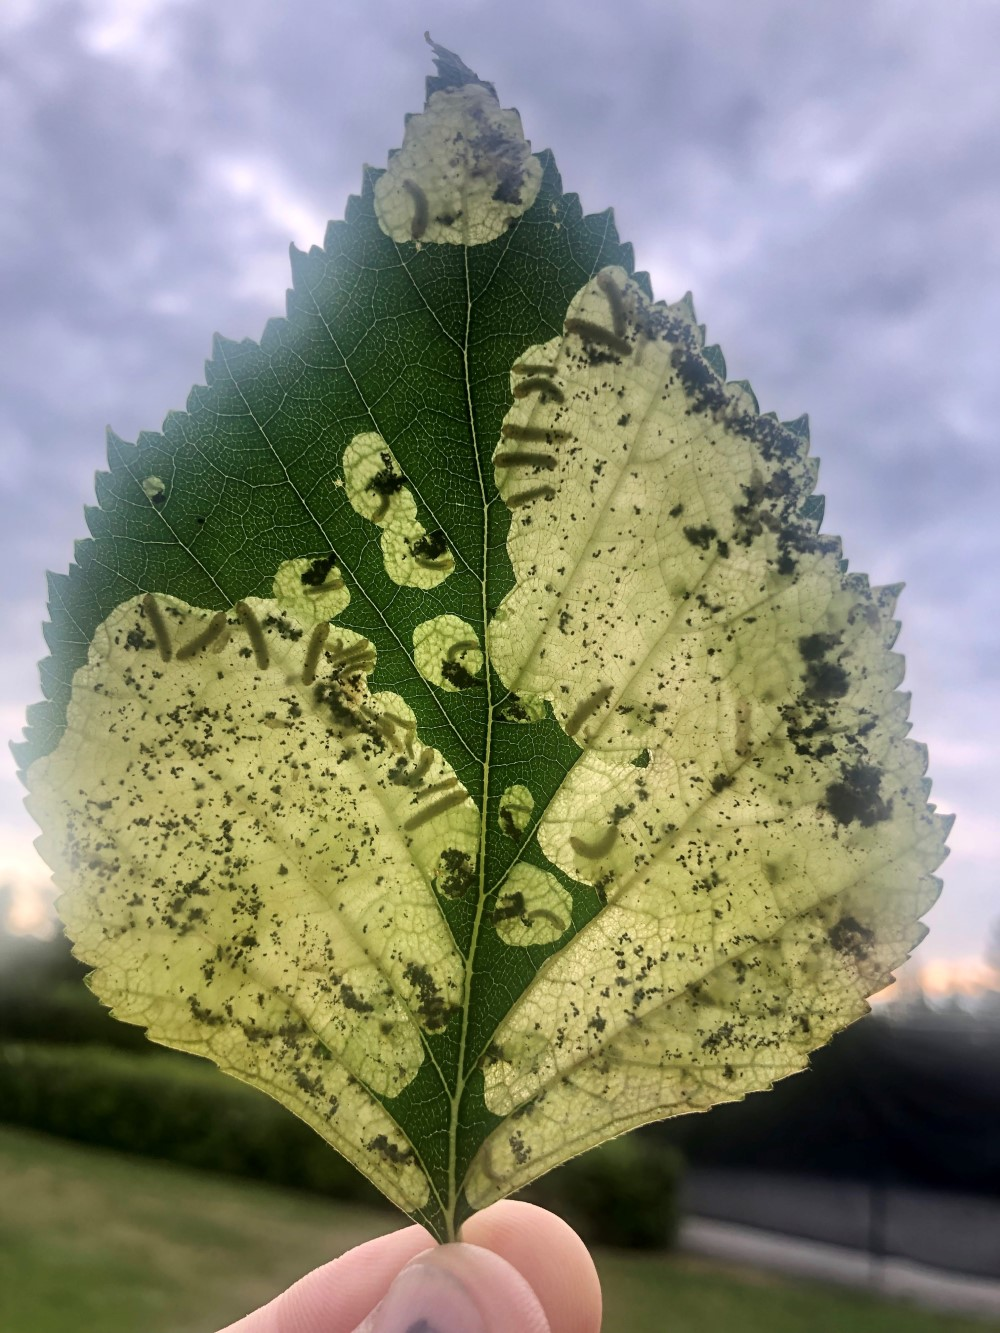
\includegraphics[width=\textwidth]{img/birch_leafminers.jpg}
\caption{Larvae of \textit{Profenusa thomsoni}, the amber marked birch leafminer collected in Fairbanks.}
\label{birch_leafminers}
\end{center}
\end{figure}  

Both birch leafminer species listed above are present in Southcentral and the Interior but the dominant species in each region differs; damage from the two cannot be distinguished to the species responsible from the air. First discovered in the late 1990’s, Southcentral populations were heavy to \textit{P.\ thomsoni}, with some \textit{H.\ nemoratus} present. Since then, population levels and severity of damage have fluctuated, and in recent years that ratio has flipped. Currently, Southcentral populations are trending toward \textit{H.\ nemoratus} as the more dominant species. Interior populations, discovered in the early 2000s, have been on the rise more recently and the majority of the population is \textit{P.\ thomsoni}. In addition to these older established populations, in 2019 a small area of birch leafminer activity was noted in the Western Kenai Peninsula Borough in the Big River Lakes area on the western side of Cook Inlet. Based on the extent of the damage in this area and its geographic isolation and separation from other known infestations of birch leafminers in the region, this appears to be a more recent introduction.

\begin{figure}[H]
\begin{center}
%\vspace{2mm}
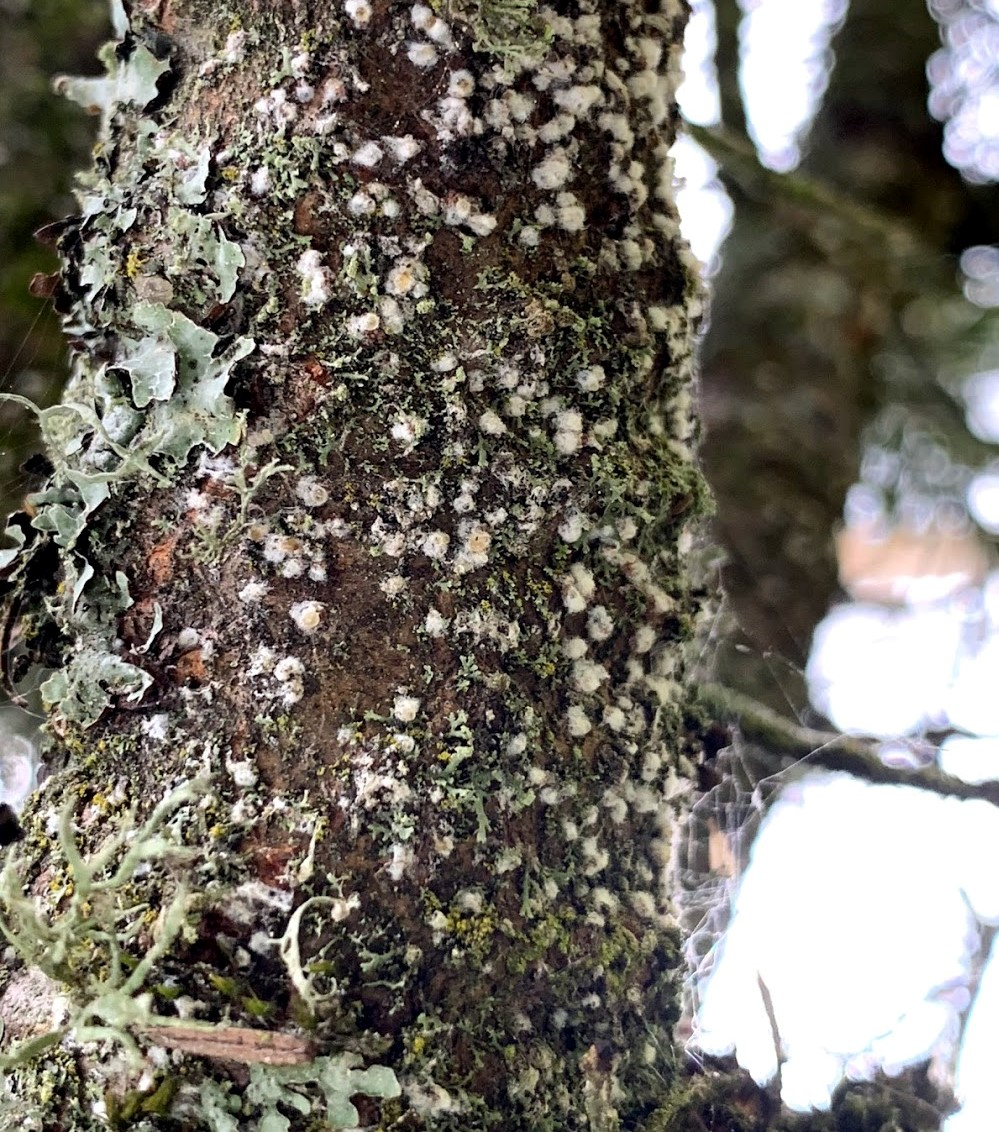
\includegraphics[width=\textwidth]{img/balsam_woolly_adelgid_on_trunk.jpg}
\caption{Balsam woolly adelgid, \textit{Adelges piceae}, on the trunk of a subalpine fir in Juneau in 2019. This recent detection is the first known occurrence of this non-native pest of true firs in Alaska.}
\label{balsam_woolly_adelgid_on_trunk}
\end{center}
\end{figure} 

\section{Balsam woolly adelgid}

The non-native balsam woolly adelgid, \textit{Adelges piceae}, was found damaging ornamental subalpine fir (\textit{Picea lasiocarpa}) in June 2019 in Juneau (Figures \ref{balsam_woolly_adelgid_on_trunk} and \ref{balsam_woolly_adelgid_adult_eggs}). This is the first known detection of this invasive species in Alaska. Balsam woolly adelgids are native to Europe and are known to occur in several other parts of the United States where they can be highly damaging to true firs. Balsam woolly adelgids are small sap-sucking insects that feed on true fir trees (\textit{Abies} spp.) and can kill a tree within a few years. Fir trees do not occur naturally in the Juneau area but are a popular ornamental tree. Subalpine fir and Pacific silver fir (\textit{Abies amabilis})  are native in nearby parts of Southeast Alaska, and balsam woolly adelgids can easily be spread over great distances by wind or wildlife. Surveys are underway to determine the extent of the infestation and funding has been made available to try and contain the threat and limit further spread.  The majority of the infested trees were located on City and Borough of Juneau property and were removed and destroyed in March 2020.  Property owners with fir trees in Juneau have been notified of this invasive species and potential treatment options. 

\begin{figure}[H]
\begin{center}
%\vspace{2mm}
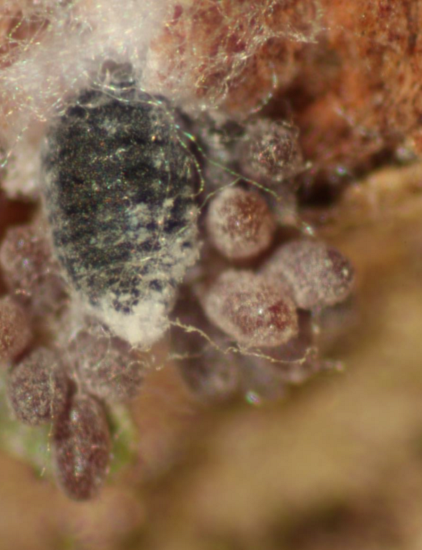
\includegraphics[width=\textwidth]{img/balsam_woolly_adelgid_adult_eggs.png}
\caption{Balsam woolly adelgid, \textit{Adelges piceae}, adult and numerous eggs.}
\label{balsam_woolly_adelgid_adult_eggs}
\end{center}
\end{figure} 
 
\section{Western Forest Insect Work Conference}

The 69\textsuperscript{th} annual Western Forest Insect Work Conference was held in Anchorage, Alaska in April 2019. This marked the first time this conference had ever occurred in Alaska. Entomologists and forest health specialists from universities, state and federal agencies, and private industry across western \acr{U.S.}\ and Canada were in attendance for the conference that featured several breakout sessions with an Alaska focus, including two sessions on spruce beetle. A joint fieldtrip with the Alaska Chapter of the Society of American Foresters took place with stops between Anchorage and Portage Lake within the Chugach National Forest. The joint fieldtrip was an excellent opportunity for entomologists and foresters to interact and discuss forest health issues with experts from different disciplines (Figure \ref{forest_insect_work_conference}).

\section{Information delivery}

\acr{USDA} Forest Service R10, Forest Health Protection has been working hard to increase timely stakeholder access to forest health information and resources: We’ve created user-friendly \acr{ESRI} ArcGIS Story Maps as a fast and fun way to learn about Forest Health Highlights in Alaska where users can explore and manipulate maps of our ground and aerial survey data. Along with the Forest Health Conditions of Alaska report, a number of other insect and disease related publications are available for viewing and download on our website: \url{https://www.fs.usda.gov/main/r10/forest-grasslandhealth}. Additionally, an interagency spruce beetle website was developed as a one-stop shop for Alaska-specific spruce beetle information to provide resources to homeowners and land managers: \url{https://www.alaskasprucebeetle.org}. This website is maintained by the University of Alaska Fairbanks Cooperative Extension Service, \acr{AKDNR} Division of Forestry and \acr{USDA} Forest Service R10, Forest Health Protection.

\bibliography{forest_highlights}

\end{multicols}
\begin{figure}[H]
\begin{center}
%\vspace{2mm}
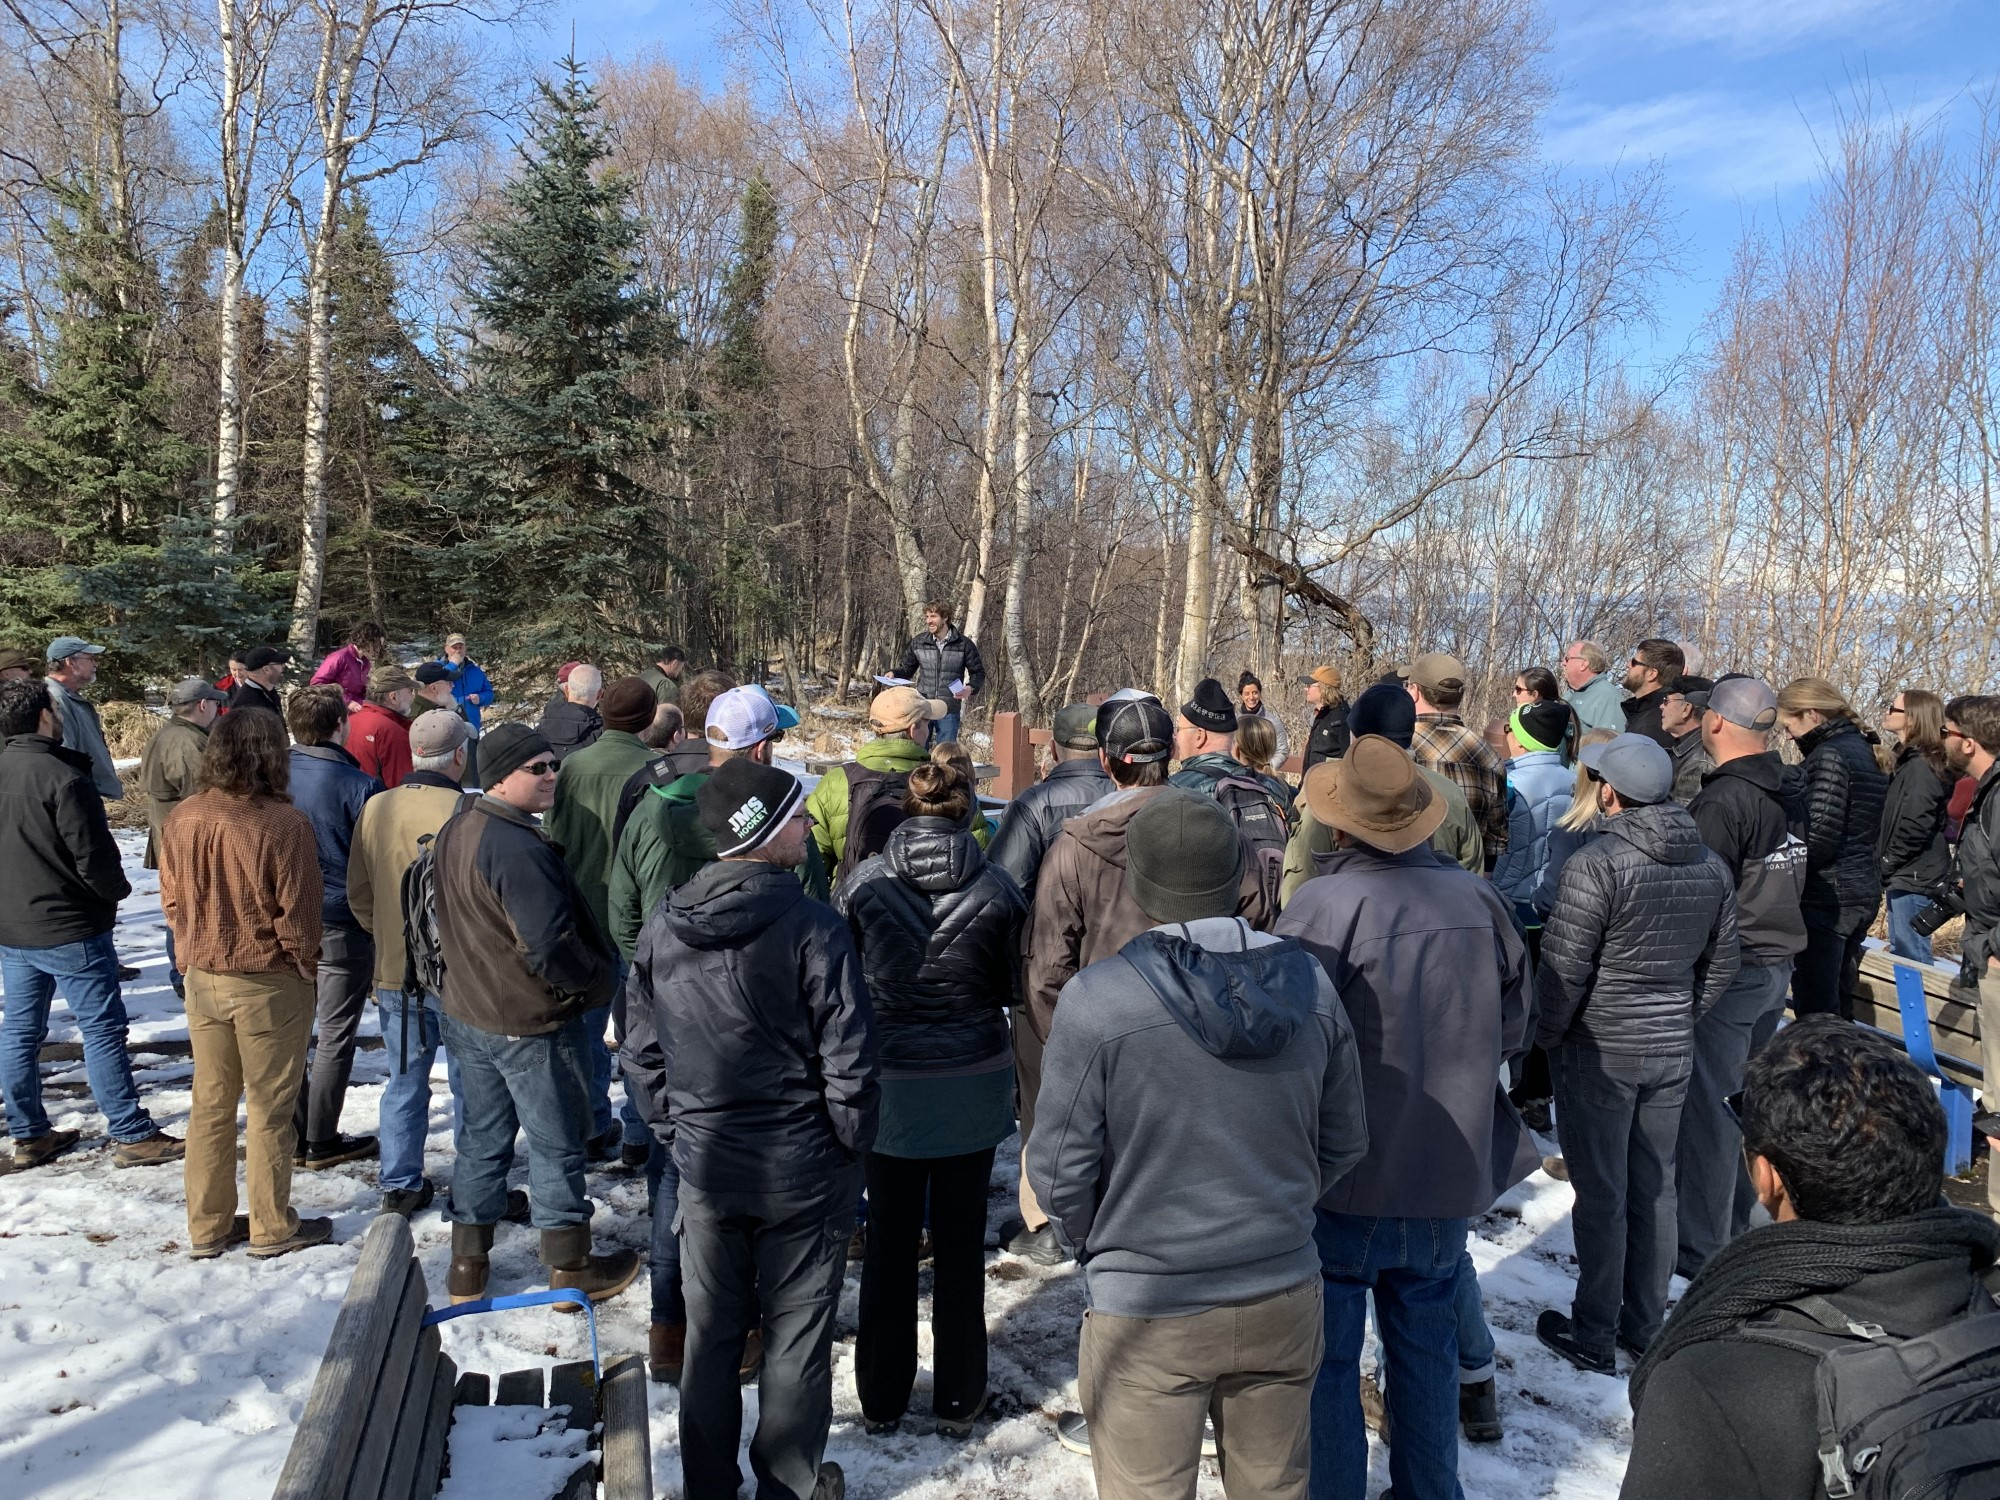
\includegraphics[width=\textwidth]{img/forest_insect_work_conference.jpg}
\caption{Gino Graziano of UAF Cooperative Extension Service addressing the Western Forest Insect Work Conference and the Alaska Chapter of the Society of American Foresters joint fieldtrip at Earthquake Park in Anchorage.}
\label{forest_insect_work_conference}
\end{center}
\end{figure} 
\begin{multicols}{2} 
